%% Template for ENG 401 reports
%% by Robin Turner
%% Adapted from the IEEE peer review template

\documentclass[journal,12pt,onecolumn,a4paper]{IEEEtran}
\usepackage{cite} % Tidies up citation numbers.
\usepackage{url} % Provides better formatting of URLs.
\usepackage[utf8]{inputenc} % Allows Turkish characters.
\usepackage{booktabs} % Allows the use of \toprule, \midrule and \bottomrule in tables for horizontal lines
\usepackage{graphicx}
\usepackage{amsmath}
\usepackage{float}
\usepackage{multicol}
\usepackage{listings}
\usepackage[numbered,framed]{matlab-prettifier}
\usepackage[export]{adjustbox}
\usepackage{titlesec}
\usepackage{hyphenat}

\graphicspath{ {./assets/pics/} }

\hyphenation{op-tical net-works semi-conduc-tor} % Corrects some bad hyphenation 
\lstset{
  basicstyle=\ttfamily,
  columns=fullflexible,
  breaklines=true,
  postbreak=\mbox{\textcolor{red}{$\hookrightarrow$}\space},
}


\begin{document}
\begin{titlepage}
	% paper title
	% can use linebreaks \\ within to get better formatting as desired
	\title{Integrasi Numerik: Table-z}


	% author names and affiliations

	\author{Adrian Ardizza - 2006524896\\
		Alya Azhar Agharid - 2006462720\\
		Muhammad Athallah - 2006527481\\
		Stefanus Ndaru Wedhatama - 2006526812
	}

	% make the title area
	\maketitle
	\begin{abstract}
		The abstract does not only mention the paper but is the original paper shrunken to approximately 200 words. It states the purpose, reports the information obtained and gives conclusions, and recommendations. In short, it summarizes the main points of the study adequately and accurately. It provides information from every major section in the body of the report in a dense and compact way. Past tense and active voice is appropriate when describing what was done. If there is any, it includes key statistical detail.

		Depending on the format you use, the abstract may come on the title page or at the beginning of the main report.

	\end{abstract}
	\tableofcontents
	\listoffigures
	\listoftables
\end{titlepage}

\IEEEpeerreviewmaketitle

\section{Pendahuluan}
Integrasi numerik adalah teknik untuk melakukan kalkulasi dan aproksimasi pada suatu nilai dengan menggunakan pendekatan metode perhitungan numerik.  Terdapat berbagai macam metode dan pendekatan baik secara integrasi numerik maupun \emph{quadrature}. Namun dalam paper ini penulis hanya akan melakukan eksplorasi dan pendekatan integrasi numerik dengan menggunakan tiga buah metode yaitu  \emph{Composite Simpson Method}, \emph{Adaptive Method}, \emph{Romberg Method}.

1. \emph{Composite Simpson Method}


2. \emph{Adaptive Method}

Adaptive Method merupakan metode perhitungan yang dapat menyelesaikan permasalahan pengambilan step-size. Step-size yang kecil cenderung akurat meski dengan time-complexity yang lebih. Namun pengambilan step-size yang wildly varying dapat berkendala.  Step-size penting untuk menemukan TOL eror.

Solusi Adaptive Quadrature menggunakan ekstraploasi dengan melalui pendekatan dengan pembagian subinterval, hal ini menyebabkan pemilihan criteria step-size dilakukan sembari kalkulasi yang sesuai. Pada penelitian ini penulis akan menggunakan Adaptive Quadrature Metode Trapezodial sebagai berikut:
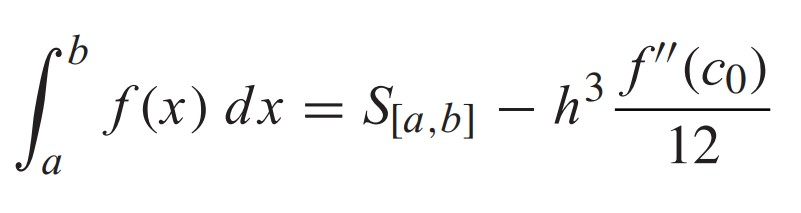
\includegraphics[scale=0.4, center]{adapt.jpg}
Untuk setiap pencarian kriterianya, akan didapatkan S[a,c]+S[c,b] dengan a<c<b pada interval [a,b] yang mengaproksimasi S[a,b]. Pengecekan dapat dilakukan antara S[a,b]-(S[a,c]+S[c,b]) hingga memenuhi kriteria 3*TOL.

(belum nambahin adaptive teori)

3. \emph{Romberg Method}
\emph{Romberg Integration} merupakan metode integrasi yang menggunakan prinsip \emph{composite trapezoidal rule} dan meningkatkan akurasi dengan melakukan ekstrapolasi melalui \emph{Richardson's Extrapolation}.

\emph{Romberg} bekerja dengan menggunakan \emph{composite trapezoidal rule} sebagai basis dari perhitungan dan melakukan iterasi dengan melakukan pembagian interval untuk meningkatkan akurasi. Basis ini diiterasi per-baris pada suatu tabel Romberg yang memiliki ukuran \(R(n,n)\) melalui rumus

\begin{equation*}
	\begin{split}
		R(1,1) & = (b-a)\frac{f(a)+f(b)}{2} \\
		R(j,1) & = \frac{1}{2}R_{j-1,1}+h_j\sum_{i=1}^{2^{j-2}}f(a+(2i-1)h_j)
	\end{split}
\end{equation*}

Jika dilihat, \(R(1,1)\) perlu diinisiasi terlebih dahulu karena untuk iterasi berikutnya, akan menggunakan hasil dari iterasi sebelumnya karena bersifat \emph{evolutionary} dengan arti meningkatkan akurasi dari iterasi sebelumnya dengan membagi interval \(h\) menjadi lebih kecil. Nilai \(h\) ini diperkecil setiap iterasi melalui rumus

\begin{equation*}
	\begin{split}
		h_j & = \frac{b-a}{2^{j-1}}
	\end{split}
\end{equation*}

Dari sini, kita bisa membentuk tabel Romberg \(R\) yang memiliki iterasi \emph{composite trapezoidal rule} dengan iterasi setiap baris, di mana semakin banyak iterasi (dan baris semakin ke bawah), maka akurasi akan semakin meningkat karena memiliki jarak interval \(h\) yang semakin kecil.

Untuk setiap baris, kita bisa menemukan akurasi yang lebih tinggi dengan mengekstrapolasi menggunakan \emph{Richardson's Extrapolation} yang mengekstrapolasi hasil dari \emph{composite trapezoidal rule} yang diperoleh. Rumus \emph{Richardson's Extrapolation} yang sudah diadaptasi untuk algoritma Romberg ini dapat dilihat sebagai berikut

\begin{equation*}
	\begin{split}
		R_{j,k} & = \frac{4^{k-1}R_{j,k-1}-R_{j-1,k-1}}{4^{k-1}-1}
	\end{split}
\end{equation*}

Dengan demikian, kita bisa mengerti bahwa algoritma Romberg melakukan integrasi dengan membangun tabel Romberg \(R\) dengan ukuran \(R(n,n)\) dan mengisi tabel tersebut sehingga membentuk \emph{lower triangular matrix} di mana setiap baris merupakan iterasi \emph{composite trapezoidal rule} dan setiap kolom merupakan peningkatan akurasi dari \emph{composite trapezoidal rule} baris tersebut menggunakan \emph{richardson's extrapolation} dengan meningkatkan \emph{order of accuracy} melalui hasil yang diperoleh pada iterasi-iterasi sebelumnya (yang akan dibahas pada \emph{subsection} toleransi eror di bawah). Dengan demikian, sebuah tabel Romberg yang dihasilkan dapat divisualisasikan sebagai berikut

\begin{center}
	\begin{tabular}{ c | c c c c c }

		j/k        & \(R(j,0)\) & \(R(j,1)\) & \(R(j,2)\) & \(R(j,3)\) & \(\cdots\) \\
		\hline
		0          & \(R(0,0)\) & -          & -          & -          & -          \\
		1          & \(R(1,0)\) & \(R(1,1)\) & -          & -          & -          \\
		2          & \(R(2,0)\) & \(R(2,1)\) & \(R(2,2)\) & -          & -          \\
		3          & \(R(3,0)\) & \(R(3,1)\) & \(R(3,2)\) & \(R(3,3)\) & -          \\
		\(\vdots\) & \(\vdots\) & \(\vdots\) & \(\vdots\) & \(\vdots\) & \(\ddots\) \\
	\end{tabular}
\end{center}

Sesuai dengan prinsip yang dijelaskan di atas, akurasi ditingkatkan dengan ekstrapolasi setiap kolomnya dengan semakin meningkat kolom (semakin ke kanan), maka hasil akan semakin akurat. Dengan demikian, nilai paling akurat untuk setiap iterasi berada pada diagonal matriks tersebut.

Hal ini menciptakan suatu sifat/fenomena konvergensi, di mana nilai hasil integrasi akan semakin konvergen menuju suatu solusi perhitungan untuk setiap diagonal yang ada. Apabila nilai diagonal sudah mencapai hasil, maka akan bersifat konvergen di mana hasil komputasi pada diagonal-diagonal sebelumnya akan mendekati nilai akhir ini, dan dengan setiap iterasi, perbedaannya akan semakin kecil antar diagonal-diagonalnya, dengan diagonal terakhir memiliki nilai paling akurat.

Maka dari itu, untuk memperoleh hasil integrasi, diambil elemen diagonal pada baris terakhir, yaitu \(R(j,j)\). Dengan demikian, dapat disimpulkan hasil integrasi melalui Romberg sebagai
\begin{equation*}
	\begin{split}
		\int_{a}^{b} f(x) \,dx & = R(j,j)
	\end{split}
\end{equation*}


Dalam paper ini, penulis diberikan sebuah fungsi probabilitas suatu variabel acak Z dengan distribusi normal kurang dari \emph{z} dengan fungsi integral berikut

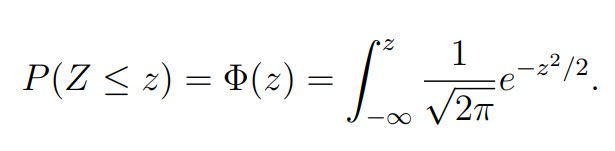
\includegraphics[scale=0.6, center]{func2.jpg}

Tujuan dari penelitian ini adalah untuk membuktikan aproksimasi nilai integral pada interval \([a, b]\) dengan ketiga metode di atas untuk menghitung probabilitas P(a kecil Z kecil B) memiliki error (perbandingan dengan nilai aktual) kurang dari \emph{TOL} yang diberikan.

\section{Implementasi Metode Composite Simpson}

\section{Implementasi Adaptive Method}
\par Fungsi yang diberikan pada distribusi normal pada persoalan tertulis sebagai berikut:
\begin{equation*}
	\begin{split}
		P(Z \le z ) & = \phi(z) = \int_{-\infty}^{z} \frac{1}{\sqrt{2\pi}}e ^{\frac{-z^2}{2}} \,dz
	\end{split}
\end{equation*}

\par Demikian pada pengerjaan pada paper ini digunakan fungsi MATLAB/Octave, sehingga fungsi distribusi normal di persoalan dapat dituliskan:
\begin{center}
	\begin{lstlisting}[language=Octave]
function res = func(z)
	res = (1/sqrt(2.*pi)).*exp((-z.^2)/2);
endfunction
	\end{lstlisting}
\end{center}

Probabilitas yang diminta untuk diselesaikan adalah
\begin{equation*}
	\begin{split}
		P(a \le Z \le b )  = \phi(a,b) & = \int_{a}^{b} \frac{1}{\sqrt{2\pi}}e ^{\frac{-z^2}{2}} \,dz
	\end{split}
\end{equation*}
Dengan begitu kita dapat melakukan translasi bentuk menyesuaikan dengan fungsi distribusi normal yang diberikan pada persoalan sebelumnya sebagai berikut:
\begin{equation*}
	\begin{split}
		P(Z \le b ) - P(Z \le a )  = \phi(b)-\phi(a) & =  \int_{-\infty}^{b} \frac{1}{\sqrt{2\pi}}e ^{\frac{-z^2}{2}} - \int_{-\infty}^{a} \frac{1}{\sqrt{2\pi}}e ^{\frac{-z^2}{2}} \,dz
	\end{split}
\end{equation*}.

Dari bentuk di atas maka akan dilakukan dua buah pemanggilan pendekatan integral yang berbeda dengan interval \([-\infty, a]\) dan interval \([-\infty, b]\). Sehingga nilai aproksimasi nilai integral keseluruhan adalah selisih dari pendekatan integrasi kedua interval tersebut.
Penulis akan menggunakan \emph{Adaptive Method} dengan \emph{Trapezoid Rule} yang mana memiliki rumus sebagai berikut:

\subsubsection{Implementasi Menggunakan Octave}

Dari penjelasan \emph{Adaptive Method} dengan \emph{Trapezoid Rule} di atas, penulis dapat menyusun sebuah algoritma pada MATLAb/Octave yaitu fungsi \emph{TrapezoidAdaptive} yang merupakan fungsi untuk pemanggilan rekursif setiap kali terjadinya pemecahan interval karena pendekatan yang masih belum mencapai batas kriteria TOL. Disusun sebagai berikut:
\begin{center}
	\begin{lstlisting}[language=Octave]
		function Q = TrapezoidAdaptive(f,a,b,Tol,ori)
		c = (a+b)/2;      % evaluate f in midpoint
		fa = f(a); fb = f(b); fc = f(c);
	  
		Q1 = (b-a)*(fa+fb)/2;        % Trapezoid rule for S[a,b]
		Q2 = (c-a)*(fc+fa)/2;        % Trapezoid rule for S[a,c]
		Q3 = (b-c)*(fb+fc)/2;        % Trapezoid rule for S[b,c]
	  
		if abs(Q1-Q2-Q3)<= 3*Tol*(b-a)/ori
		  Q = Q2+Q3;   %accept trapezoid rule value
		else
		  Q = TrapezoidAdaptive(f, a,c, Tol/2, ori) + TrapezoidAdaptive(f,c,b, Tol/2, ori); % use algorithm for [a,c] and [c,b]
		end
	  end
	\end{lstlisting}
\end{center}

\subsubsection{Analisis Hasil Komputasi pada Octave}

Untuk melihat hasil implementasi, akan digunakan input dengan spesifikasi berikut

\begin{center}
	\begin{lstlisting}[language=Octave]
		minInf = -1e4;
		a = input('Masukkan batas bawah interval a:  ');
		b = input('Masukkan batas atas interval b:  ');
		TOL = input('Masukkan Tolerance TOL:  ');

		orig = b-a;
		printf("\nP(Z <= a)\n")
		Pa = TrapezoidAdaptive(@func,minInf,a,TOL,orig)

		printf("\nP(Z <= b)\n")
		Pb = TrapezoidAdaptive(@func,minInf,b,TOL,orig)

		approx = Pb-Pa
		printf("\nHasil Aproksimasi Integrasi: %d\n", approx)
	\end{lstlisting}
\end{center}

Pada fungsi pengerjaan yang dibangun di atas, penulis menggunakan asumsi untuk penggunaan bilangan \(-\infty\) disubstitusikan dengan bilangan yang sangat kecil dalam fungsi di atas atau digunakan nilai \lstinline{1e-4} pada variabel minInf. Dikarenakan Adaptive Method merupakan fungsi rekursi, maka dengan batas bawah \(-\infty\) atau dengan bilangan yang lebih kecil dari \lstinline{1e-4} akan menimbulkan error max depth recursion.
Seperti apa yang sudah dirumuskan pada bagian sebelumnya, akan dilakukan dua buah pemanggilan dengan interval yang berbeda yang nilai aproksimasi masing-masing interval akan disimpan pada variabel \(Pa\) dan \(Pb\). Hasil integrasi yang memenuhi persamaan \(P(a \le Z \le b)\) adalah dengan hasil selisih kedua pendekatan di atas \(P(Z \le b ) - P(Z \le a )\).

Untuk kasus dengan spesifikasi input batas bawah \emph{a = -1} dan batas atas \emph{b = 1.0} akan menghasilkan \emph{output} dengan dua kali pemanggilan fungsi dengan interval berbeda sebagai berikut:

\begin{center}
	\begin{lstlisting}[language=Octave]
		Masukkan batas bawah interval a:  -1
		Masukkan batas atas interval b:  1
		Masukkan Tolerance TOL:  0.0001

		P(Z <= a)
		Pa = 0.158655267050648

		P(Z <= b)
		Pb = 0.841344747955897
		approx = 0.682689480905249

		Hasil Aproksimasi Integrasi: 0.682689480905249

	\end{lstlisting}
\end{center}

Hal ini dapat dibandingkan dengan pemanggilan fungsi secara langsung untuk perhitungan integrasi pemanggilan \(P(a \le Z \le b)\), dilakukan komputasi dan hasil sebagai berikut:
\begin{center}
	\begin{lstlisting}[language=Octave]
		integ = TrapezoidAdaptive(@func,a,b,TOL,orig);
		printf("\nHasil Aproksimasi Integral P(a<=Z<=b): %d\n", integ)

		Hasil Aproksimasi Integral P(a<=Z<=b): 0.682689173963903
	\end{lstlisting}
\end{center}

Hasil percobaan di atas antara pemanggilan fungsi dengan integrasi pemanggilan \(P(a \le Z \le b)\) dengan \(P(Z \le b ) - P(Z \le a )\) memiliki hasil yang demikian serupa yakni dengan hasil \(P(a \le Z \le b)= 0.682689480905249\)  dan \(P(Z \le b ) - P(Z \le a ) = 0.682689480905249\). Perbandingan eror kedua hasil integrasi adalah sebagai berikut:

\begin{center}
	\begin{lstlisting}[language=Octave]
	printf("\nBeda Hasil Komputasi P(a <= Z <= b) dan P(Z <= b) - P(Z <= a)\n")
	diff_res = approx - integ

	Beda Hasil Komputasi P(a <= Z <= b) dan P(Z <= b) - P(Z <= a)
	diff_res = 3.069413463396842e-07
	\end{lstlisting}
\end{center}

Dengan tingkat perbedaan pada angka \lstinline{1e-07}, penulis dapat mengatakan kedua implementasi dapat digunakan dan memiliki hasil perhitungan yang demikian sama. Yang menjadi pembeda antara kedua cara komputasi di atas adalah waktu komputasi untuk pemanggilan pendekatan satu integrasi dengan interval \([a,b]\) dan dengan interval \([-\infty,b] dan [-\infty,b]\) yang menggunakan dua pemanggilan integral. Maka pengerjaan \(P(Z \le b ) - P(Z \le a )\) memiliki waktu komputasi lebih lama karena selain mengeksekusi dua integrasi juga integrasi yang dieksekusi menghitung dari batas bawah \(-\infty\) atau dalam komputasi di atas adalah \lstinline{1e-4}.

\subsection{Toleransi Error}

\emph{Adaptive Method} dengan aturan Trapezoid dan aturan titik tengah akan mengatur pembagian subinterval menyesuaikan fungsi yang diintegrasi pada interval tertentu dan kebutuhan akurasi. Karena dilakukan untuk setiap subinterval, eror global tidak diketahui dan dibutuhkan pendekatan eror yang diketahui bahwa kita dapat mengatur nilai eror adalah

\begin{equation*}
	\begin{split}
		E  = \frac{T(f) - M(f)}{3}
	\end{split}
\end{equation*}

Adapun diketahui bentuk dari \emph{composite trapezoidal rule}, yaitu:
\begin{equation*}
	\begin{split}
		\int_{a}^{b} f(x) \,dx & = \frac{h}{2}[y_0+y_m+2\sum_{j=1}^{m-1}f(y_i)]-\frac{(b-a)h^2}{12}f^(2)(c)
	\end{split}
\end{equation*}

Dari sini kita bisa lihat bahwa \emph{trapezoidal rule} mencapai batas akurasi paling tinggi berupa \(O(^2)\). Dengan jika komputasi batas E terlalu besar dan tidak mencapai kriteria, maka interval dapat dipecah dari \([a,b]\) menjadi \([a,c]\) dan \([c,b]\) dengan \emph{c} adalah nilai tengah kedua batas integral.
Operasi interasi tersebut akan diulangi hingga besar E memenuhi batas yag dikehendaki.
Dengan begitu kombinasi aturan eror pada dua tingkat metode trapezoid untuk \emph{Adaptive Method} adalah sebagai berikut:

\begin{equation*}
	\begin{split}
		T_{h}(f) & = I(f) + O(h^2) \\
		T_{h/2}(f) & = I(f) + \frac{1}{4}O(h^2)
	\end{split}
\end{equation*}

(tolong bantuin gua toleransi error aijfhijdiadj)



Pembuktian melalui eksekusi percobaan pada bagian sebelumnya, penulis membandingkan hasil aproksimasi dengan pendekatan metode Adaptive dengan nilai aktual integrasi melalui beberapa fungsi bawaan Octave dan metode pencocokan dengan nilai probabilitas tabel-Z yang sesungguhnya.

1. Percobaan dengan fungsi \lstinline{quadgk}, yang merupakan fungsi integrasi Octave dengan algoritma \emph{adaptive Gauss-Konrod quadrature}.\lstinline{Quadgk} tergolong ke dalam fungsi yang memiliki \emph{Medium accuracy (1e-6 - 1e-9) with smooth integrands}. Fungsi ini menangani fungsi yang osilasi dan dengan batas integrasi tak hingga seperti pada persoalan di atas. Implementasi perbandingan hasil integrasi aproksimasi interval \([-1,1]\) pengerjaan dan \lstinline{quadgk} adalah sebagai berikut:
\begin{center}
	\begin{lstlisting}[language=Octave]
		[quadAns, err] = quadgk(@func, a, b)
		err_quad = abs(quadAns-approx);
		err_quad_ab = abs(quadAns-integ);
		printf("----------")
		printf("\nHasil Aktual dengan Metode Quadgk: %d\n", quadAns)
		printf("\nEror P(Z <= b) - P(Z <= a)  Vs. Metode Quadgk: %d\n", err_quad)
		printf("\nEror P(a <= Z <= b) Vs. Metode Quadgk: %d\n", err_quad_ab)
	\end{lstlisting}
\end{center}

dengan hasil sebagai berikut

\begin{center}
	\begin{lstlisting}[language=Octave]
		Hasil Aktual dengan Metode Quadgk: 
		quadAns = 0.682689492137086
		err = 4.795122632295090e-14  

		Eror P(Z <= b) - P(Z <= a)  Vs. Metode Quadgk: 1.123183701601249e-08
		Eror P(a <= Z <= b) Vs. Metode Quadgk: 3.181731833556967e-07
	\end{lstlisting}
\end{center}

\lstinline{Quadgk} memiliki akurasi dan error \lstinline{1e-14} yang terbilang cukup akurat dan memiliki perbedaan akurasi dengan hasil aproksimasi sebanyak \lstinline{1e-7} dan \lstinline{1e-8}. Hal ini membuktikan aproksimasi dengan metode Adaptive yang menerapkan aturan Trapezoid masih memiliki perbedaan akurasi yang lumayan, tetapi tidak dapat dikatakan buruk. Hal ini juga bergantung pada nilai besar TOL yang ditentukan.


2. Percobaan dengan fungsi \lstinline{normcdf} yang merupakan suatu fungsi distribusi normal. Dengan begitu membandingkan hasil aproksimasi metode ini dengan \lstinline{normcdf} akan dirasa lebih akurat dengan membandingkannya pada fungsi distribusi normal langsung.

\begin{center}
	\begin{lstlisting}[language=Octave]
		cdf = normcdf([a b]);
		cdf_ans = cdf(2) - cdf(1);
		err_cdf = abs(cdf - approx);
		err_cdf_ab = abs(cdf - integ);

		printf("----------")
		printf("\nHasil NormCDF for Z value (Actual Value)\n: %d", cdf_ans)
		printf("\nEror P(Z <= b) - P(Z <= a)  Vs. Metode NormCDF: %d\n", err_cdf)
		printf("\nEror P(a <= Z <= b) Vs. Metode NormCDF: %d\n", err_cdf_ab)
	\end{lstlisting}
\end{center}

dengan hasil sebagai berikut

\begin{center}
	\begin{lstlisting}[language=Octave]
		Hasil NormCDF for Z value (Actual Value): 0.682689492137086
		Eror P(Z <= b) - P(Z <= a)  Vs. Metode NormCDF: 1.123183690499019e-08
		Eror P(a <= Z <= b) Vs. Metode NormCDF: 3.181731832446744e-07
	\end{lstlisting}
\end{center}

Keluaran perbandingan nilai aproksimasi integrasi percobaan ini dengan fungsi \lstinline{quadgk} dan \lstinline{normcdf} memiliki besar perbedaan nilai
yang hampir serupa di atas yaitu untuk \(P(a \le Z \le b)= 1.123183690499019e-08\)  dan \(P(Z \le b ) - P(Z \le a ) = 3.181731832446744e-07\).
Dengan begitu dapat dikatakan fungsi aproksimasi dengan metode
Adaptive Trapezoid ini sudah cukup akurat menyesuaikan dengan fungsi bawaan Octave yaitu \lstinline{quadgk} dan utamanya \lstinline{normcdf} yang merupakan fungsi distribusi normal.

Percobaan di atas jika dijalankan dengan serangkaian TOL yang berbeda juga akan menghasilkan hasil error pembanding dengan \lstinline{quadgk} dan \lstinline{normcdf} di atas, digambarkan pada grafik di bawah.
(Percobaan dengan interval \([0,0.01]\))
\begin{figure}[h]
	\centering
	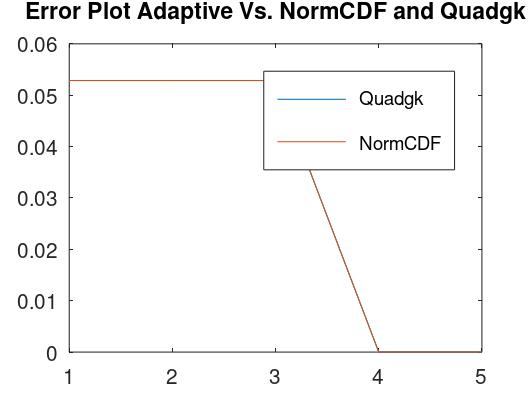
\includegraphics[width=0.5\textwidth]{trapezoid graf.jpg}
	\caption{Grafik Nilai Eror Hasil Komputasi Adaptive dengan fungsi bawaan (quadgk dan normcdf)}
	\label{fig:difGraphAdaptive}
\end{figure}

Dengan begitu percobaan aproksimasi metode Adaptive dengan aturan Trapezoid mengeluarkan hasil yang sesuai dan memiliki akurasi yang sesuai serta menyesuaikan dengan TOL eror yang diberikan. Hasil komputasi juga sesuai atau mendekati dengan fungsi distribusi normal dan hasil integrasi aktual fungsi bawaan.

\subsection{Analisis Kompleksitas}
Berikut dilakukan perhitungan FLOP (\emph{floating-point operatons}) pada implementasi kode.

\begin{center}
	\begin{lstlisting}[language=Octave]
if tol < 1e-14
	printf("Tolerance is too small and will produce errors, please use larger values\n")
	res = 0;
	return;
endif

n = 100;
R = zeros(n, n);
R(1,1) = (b-a)*(f(a)+f(b))/2;
	\end{lstlisting}
\end{center}

Di sini, terdapat 5 FLOPs yang terjadi, yaitu pada kondisi toleransi, dan inisiasi elemen pertama \\ \lstinline{R(1,1)}. Lanjut analisis ke dalam \emph{loop}
\begin{center}
	\begin{lstlisting}[language=Octave]
		function Q = TrapezoidAdaptive(f,a,b,Tol,ori)
			c = (a+b)/2;      % evaluate f in midpoint
			fa = f(a); fb = f(b); fc = f(c);

			Q1 = (b-a)*(fa+fb)/2;        % Trapezoid rule for S[a,b]
			Q2 = (c-a)*(fc+fa)/2;        % Trapezoid rule for S[a,c]
			Q3 = (b-c)*(fb+fc)/2;        % Trapezoid rule for S[b,c]

			if abs(Q1-Q2-Q3)<= 3*Tol*(b-a)/ori
				Q = Q2+Q3;   %accept trapezoid rule value
			else
				Q = TrapezoidAdaptive(f,a,c,Tol/2,ori) + TrapezoidAdaptive(f,c,b,Tol/2,ori);
				% use algorithm for [a,c] and [c,b]
			end
		end
	\end{lstlisting}
\end{center}

(belum analisis kompleksitas algoritma)

\subsection{Implementasi Algoritma Romberg}

\subsubsection{Implementasi Menggunakan Octave}

\par Untuk tugas kelompok kedua ini, diberikan fungsi distribusi normal tabel Z sebagai berikut
\begin{equation*}
	\begin{split}
		P(Z \le z ) & = \phi(z) = \int_{-\infty}^{z} \frac{1}{\sqrt{2\pi}}e ^{\frac{-z^2}{2}} \,dz
	\end{split}
\end{equation*}

Pada TK ini, kami diminta untuk mengimplementasikan semua algoritma pada MATLAB/Octave. Maka dari itu, dibentuk implementasi dalam Octave untuk fungsi distribusi normal tersebut

\begin{center}
	\begin{lstlisting}[language=Octave]
function ret = zNormalDist(z)
	ret = (1/sqrt(2.*pi)).*exp((-z.^2)/2);
endfunction
	\end{lstlisting}
\end{center}

Berdasarkan penjelasan algoritma Romberg, kita bisa mengetahui bahwa dalam implementasinya, kita hanya perlu memanggil fungsi yang ingin diintegralkan. Dalam kasus ini, fungsi tersebut adalah fungsi distribusi normal yang sudah disebutkan di atas. Karena fungsi tersebut sudah dibuat implementasi Octavenya, maka kita hanya perlu membuat fungsi Romberg yang menerima fungsi distribusi normal tersebut. Implementasi algoritma Romberg dalam Octave merupakan translasi langsung dari rumus yang sudah disebutkan pada bagian sebelumnya, sehingga bisa diimplementasikan sebagai berikut
\begin{center}
	\begin{lstlisting}[language=Octave]
function [res, R, j] = rombergIntegration(a, b, tol, f)

if tol < 1e-14
	printf("Tolerance is too small and will produce errors, please use larger values\n")
	res = 0;
	return;
endif

n = 100;
R = zeros(n, n);
R(1,1) = (b-a)*(f(a)+f(b))/2;

for j = 2:n
	h = (b-a)/2^(j-1);
	Rval = 0;

	for i = 1:2^(j-2)
		Rval = Rval + f(a+(2*i - 1)*h);
	endfor

		R(j,1) = (1/2)*R(j-1,1) + h*Rval;

	for k = 2:j
		topval = 4^(k-1)*R(j,k-1) - R(j-1,k-1);
		botval = 4^(k-1) - 1;
		R(j,k) = topval/botval;
	endfor

	if abs(R(j,j)-R(j-1,j-1)) < tol
		break;
	endif

endfor

R(1:j,1:j);
res = R(j,j);

endfunction
	\end{lstlisting}
\end{center}

Jika diperhatikan, fungsi ini memang hanya merupakan translasi dari rumus yang sudah diberikan. Perbedaannya, pada implementasi ini, tabel Romberg sudah didefinisikan dengan ukuran \(R(100,100)\). Hal ini dilakukan berdasarkan asumsi di mana hasil komputasi tidak akan mencapai baris dan kolom ke-100 karena sifat Romberg yang menggunakan ekstrapolasi untuk mencari nilai paling akurat, sehingga seharusnya, berdasarkan asumsi, tidak akan memakan komputasi sebanyak itu.

Selain itu, diberikan juga \emph{guard} berupa batas toleransi maksimum dari perhitungan. Di awal, diberikan batas toleransi berupa \lstinline{tol < 1e-14} yang berarti toleransi maksimum diperbolehkan hanya mencapai \lstinline{1e-13}. Hal ini dikarenakan fungsi referensi untuk perhitungan integral dari Octave yang akan digunakan pada laporan ini, yaitu \emph{quadgk}, memiliki batas toleransi mencapai \lstinline{1e-14} sebagai nilai terendah dari hasil percobaan kami.

Ditambah pula, apabila nilai toleransi terlalu rendah, maka adanya kemungkinan terjadi error yang diakibatkan oleh limitasi komputasi oleh Octave yang dapat mengakibatkan hasil komputasi yang tidak akurat. Agar hal itu tidak terjadi, maka dibuatlah kondisi ini.

Toleransi maksimum juga ada di bagian bawah setelah iterasi kolom, yaitu ketika iterasi mencapai sel diagonal pada matriks. Apabila mencapai diagonal, sesuai pembahasan di atas, maka telah tercapai nilai paling akurat untuk iterasi tersebut. Di sini, akan diperiksa perbedaan antar diagonalnya melalui \(|R(n,n)-R(n-1,n-1)| < tol\). Seperti yang di bahas di atas, terjadi fenomena konvergensi pada diagonal di mana perbedaan antar diagonal menjadi semakin kecil dan semakin mendekati hasil akhir yang dituju. Ketika perbedaan ini sudah sangat kecil di bawah batas toleransi yang diinginkan, maka tidak ada tujuan lain untuk melanjutkan iterasi sehingga iterasi dihentikan.

Dengan demikian, fungsi tersebut akan menerima beberapa input berupa batas bawah integrasi, batas atas integrasi, batas toleransi yang diinginkan, dan fungsi yang akan di-\emph{pass}, dalam kasus ini adalah fungsi distribusi normal.

\subsubsection{Hasil Komputasi pada Octave}

Untuk menentukan hasil implementasi, akan digunakan input dengan spesifikasi berikut

\begin{center}
	\begin{lstlisting}[language=Octave]
minInf = -1e3;
low = -1;
high = 3;
tol = 1e-7;

printf("\nKalkulasi z-Score Integration dengan Romberg")
printf("\nDengan spesifikasi sebagai berikut:")
printf("\nLower Limit: %d", low)
printf("\nUpper Limit: %d", high)
printf("\nTolerance Limit: %d\n\n", tol)
	\end{lstlisting}
\end{center}

Jika dilihat, nilai \lstinline{minInf} akan menggunakan \lstinline{1e-3}. Hal ini dikarenakan penggunaan nilai yang lebih kecil akan memakan komputasi lebih lama karena implementasi yang dilakukan akan menghitung dari nilai bawah yang sangat kecil tersebut. Selain itu, hasil komputasi fungsi distribusi normal di atas akan memiliki nilai yang sangat kecil untuk \(x \le -100\) sehingga akan menjadi \emph{redundant} dan perbedaan akan tidak terlalu signifikan. Hal ini akan ditunjukkan pada contoh eksekusi implementasi kode di bawah.

Lalu, fungsi integrasi Romberg akan dipanggil dua kali untuk melihat 2 cara dari 2 pemanggilan/komputasi berbeda untuk distribusi normal. Sebelumnya, perlu diketahui bahwa fungsi distribusi normal bisa dihitung dengan dua cara. Misalkan kita ingin memanggil untuk suatu interval \(P(a \le Z \le b)\). Maka, bisa didefinisikan sebagai

\begin{equation*}
	\begin{split}
		P(a \le Z \le b )  = \phi(a,b) & = \int_{a}^{b} \frac{1}{\sqrt{2\pi}}e ^{\frac{-z^2}{2}} \,dz \\
		=  P(Z \le b ) - P(Z \le a )  = \phi(b)-\phi(a) & =  \int_{-\infty}^{b} \frac{1}{\sqrt{2\pi}}e ^{\frac{-z^2}{2}} - \int_{-\infty}^{a} \frac{1}{\sqrt{2\pi}}e ^{\frac{-z^2}{2}} \,dz
	\end{split}
\end{equation*}

Dengan demikian, dapat diimplementasikan pada Octave untuk kedua pemanggilan tersebut

\begin{center}
	\begin{lstlisting}[language=Octave]
printf("\nHasil Integrasi dengan P(a <= Z <= b)\n")

[res, R, j] = rombergIntegration(low, high, tol, @zNormalDist);
R(1:j,1:j)
res

printf("\nHasil Integrasi dengan P(Z <= b) - P(Z <= a)\n")

[res1, R1, j1] = rombergIntegration(minInf, low, tol, @zNormalDist);
res1

[res2, R2, j2] = rombergIntegration(minInf, high, tol, @zNormalDist);
res2

printf("\n")
ansMinInf = abs(res2-res1)
	\end{lstlisting}
\end{center}

Dengan \lstinline{R(1:j,1:j)} adalah tabel Romberg dan \lstinline{res} adalah hasil komputasi untuk pemanggilan \(rombergIntegration\). Untuk memperoleh hasil melalui cara \(P(Z \le b ) - P(Z \le a )\), maka akan dikomputasi melalui pengurangan dan variabel \lstinline{ansMinInf}. Untuk kasus dengan spesifikasi di atas, akan menghasilkan \emph{output}

\begin{center}
	\begin{lstlisting}[language=Octave]
Hasil Integrasi dengan P(a <= Z <= b)
ans =

Columns 1 through 3:

0.492805145862163   0                   
0.730344021969368   0.809523647338437   0
0.818105257899305   0.847359003209284   0.849881360267340
0.834640903793682   0.840152785758475   0.839672371261754
0.838663131013866   0.840003873420594   0.839993945931402
0.839662332840927   0.839995400116614   0.839994835229682
0.839911744979600   0.839994882359158   0.839994847841994

Columns 4 through 6:

0
0
0 
0.839510323817221	0
0.839999050291238	0.840000966865646	0
0.839994849345527	0.839994832871231	0.839994826875146
0.839994848042189	0.839994848037078	0.839994848051903

Column 7:

0
0
0
0
0
0
0.839994848057074

res = 0.839994848057074

Hasil Integrasi dengan P(Z <= b) - P(Z <= a)
res1 = 0.158655253936076
res2 = 0.998650101990628

ansMinInf = 0.839994848054551
	\end{lstlisting}
\end{center}

Dapat dilihat bahwa keduanya menghasilkan nilai yang cukup dekat antara satu dengan yang lainnya, dengan \(P(a \le Z \le b)= 0.839994848057074\)  dan \(P(Z \le b ) - P(Z \le a ) = 0.839994848054551\). Jika kita ingin melihat lebih detail, keduanya memiliki perbedaan sebagai berikut, dengan implementasi Octave dan hasilnya

\begin{center}
	\begin{lstlisting}[language=Octave]
printf("\nPerbedaan Antara P(a <= Z <= b) dan P(Z <= b) - P(Z <= a)\n")
diff = res - ansMinInf

Perbedaan Antara P(a <= Z <= b) dan P(Z <= b) - P(Z <= a)
diff = 2.522870801158206e-12
	\end{lstlisting}
\end{center}

Dapat dilihat bahwa perbedaannya sangat kecil, dengan tingkat perbedaan pada angka \lstinline{1e-12} sehingga bisa dibilang keduanya memiliki perbedaan yang insiginifikan dan salah satu dari kedua implementasi bisa digunakan. Tetapi, perlu diketahui bahwa metode \(P(Z \le b ) - P(Z \le a )\) akan memakan waktu komputasi lebih lama karena harus menghitung dari batas bawah \lstinline{-inf}, yang pada implementasi ini berupa \lstinline{-1e3} sehingga memakan \emph{resource} yang lebih besar. Maka, jika kita ingin menghitung pada interval \([a,b]\), lebih baik menggunakan implementasi \(P(a \le Z \le b)\).

\subsection{Toleransi Error}
Seperti yang diimplementasikan di atas, fungsi Romberg akan mengalami konvergensi pada setiap diagonal hingga mencapai nilai hasil integrasi yang paling akurat. Hal ini terjadi karena adanya iterasi \emph{composite trapezoidal rule} dan \emph{richardson's extrapolation}. Untuk lebih memahami bagaimana iterasi trapezoid dan ekstrapolasi ini meningkatkan akurasi, perlu dilihat analisis berdasarkan \emph{order of accuracy}. Pembahasan toleransi eror akan menggunakan sumber referensi dari \cite{jim_lamber}.

Pertama-tama, kita perlu mengetahui bentuk umum dari \emph{composite trapezoidal rule}, yaitu
\begin{equation*}
	\begin{split}
		\int_{a}^{b} f(x) \,dx & = \frac{h}{2}[f(a)+2\sum_{j=1}^{n-1}f(x_j)+f(b)]+\sum_{i=1}^{\infty}K_ih^{2i}
	\end{split}
\end{equation*}

dengan \(h=\frac{b-a}{n}, x_j = a+jh\), dan konstanta \({K_i}_{i=1}^{\infty}\) bergantung kepada turunan dari fungsi \(f(x)\). Dapat dilihat bahwa akurasi dapat ditingkatkan dengan \emph{richardson's extrapolation}, dan ini yang dilakukan pada algoritma Romberg.
Jika kita nyatakan \(I(f)\) sebagai hasil komputasi integrasi, maka pada tabel Romberg kita bisa peroleh

\begin{equation*}
	\begin{split}
		T_{1,1} & = I(f) + K_1h^2 +O(h^4) \\
		T_{2,1} & = I(f) + K_1(\frac{h}{2})^2 + O(h^4)
	\end{split}
\end{equation*}

Dari sini kita bisa lihat bahwa \emph{composite trapezoidal rule} mencapai batas akurasi paling tinggi berupa \(O(h^4)\), yang artinya akurasi hanya mencapai derajat 4 atau \(10^{-4}\).
Sekarang kita akan melanjutkan iterasi dan komputasi aproksimasi \(T_{2,2}, T_{3,1}, T_{3,2}\) menggunakan \emph{composite trapezoidal rule} untuk baris, lalu untuk kolom akan digunakan \emph{richardson's extrapolation}. Maka, akan diperoleh
\begin{equation*}
	\begin{split}
		T_{2,2} & = I(f) + \tilde{K}_2h^4 +O(h^6) \\
		T_{3,2} & = I(f) + \tilde{K}_2(\frac{h}{2})^4 + O(h^6)
	\end{split}
\end{equation*}

Dapat dilihat bahwa akurasi meningkat hingga \(O(h^6)\), yang artinya akurasi mencapai derajat 6 atau \(10^{-6}\). Hal ini disebabkan oleh adanya ekstrapolasi yang meningkatkan akurasi dengan pertumbuhan akurasi \(O(h^{2k+2})\) dengan \(k\) adalah kolom ke-\(k\). Dengan demikian, semakin banyak iterasi, eror akan semakin besar, dengan akurasi terbaik berada pada elemen diagonal akibat pertumbuhan akurasi akibat ekstrapolasi.
Selain itu, karena akurasi semakin meningkat dan eror semakin kecil, maka dengan setiap iterasi, nilai akan semakin mendekati hasil eksak dan akan terjadi fenomena konvergensi dengan perbedaan antar nilai, terutama pada diagonal, semakin kecil.

Dengan premis ini, algoritma Romberg yang diimplementasikan akan memanfaatkan peningkatan akur\hyp{}asi dan juga sifat konvergensi untuk menentukan kapan algoritma berhenti sesuai dengan toleransi eror. Implementasi ini dilakukan melalui \lstinline{if abs(R(j,j)-R(j-1,j-1)) < tol} yang menghitung perbedaan elemen diagonal \(|R(n,n)-R(n-1,n-1)| < tol\) di mana jika perbedaan sudah lebih kecil daripada toleransi, maka akan berhenti.
Hal ini menjamin nilai yang diperoleh akan memiliki akurasi di bawah batas toleransi yang diberikan karena nilai yang berbeda dan masih dalam proses konvergensi berada di luar batas, sementara nilai yang masuk batas toleransi sudah dijamin konvergen dan merupakan nilai akhir hasil komputasi.

Berdasarkan contoh eksekusi pada bagian sebelumnya, kita bisa membuktikan hasil implementasi kita melalui perbandingan hasil dengan hasil komputasi integrasi aktual dari fungsi bawaan Octave.

Fungsi pertama yang akan diuji adalah menggunakan fungsi \lstinline{quadgk}, yaitu fungsi integrasi dari Octave menggunakan algoritma \emph{adaptive Gauss-Konrod quadrature}. Menurut Octave, \lstinline{quadgk}, memiliki karakteristik \emph{Medium accuracy (1e-6 - 1e-9) with smooth integrands. Handles oscillatory functions and infinite bounds}, dan memiliki tingkat akurasi yang lebih baik daripada fungsi integrasi satu variabel lain seperti \lstinline{quad, quadv, dan quadl} yang menjadi alasan kami menggunakan fungsi ini sebagai referensi.
Perbandingan ini diimplementasikan sebagai berikut

\begin{center}
	\begin{lstlisting}[language=Octave]
printf("\n\nHasil Integrasi dengan quadgk\n")
[quadgkAns, err] = quadgk(@zNormalDist, low, high)

printf("\n\nError dengan Hasil Integrasi melalui quadgk\n")
err1 = abs(quadgkAns - res);
err2 = abs(quadgkAns - ansMinInf);
printf("\nP(a <= Z <= b): %d", err1)
printf("\nP(Z <= b) - P(Z <= a): %d", err2)
	\end{lstlisting}
\end{center}

dan menghasilkan hasil berupa

\begin{center}
	\begin{lstlisting}[language=Octave]
Hasil Integrasi dengan quadgk
quadgkAns = 0.839994848036913
err = 5.904228928682587e-14

Error dengan Hasil Integrasi melalui quadgk

P(a <= Z <= b): 2.01614e-11
P(Z <= b) - P(Z <= a): 1.76386e-11
	\end{lstlisting}
\end{center}

dari sini, kita bisa melihat bahwa \lstinline{quadgk} memiliki akurasi dan error dalam tingkat \lstinline{1e-14} sehingga bisa dibilang cukup akurat. Pada implementasi Romberg, diberikan spesifikasi batas toleransi \lstinline{1e-7}, tetapi dari perbandingan di atas, tingkat perbedaan yang menunjukan eror berada pada derajat 11 atau \lstinline{1e-11}.
Hal ini menandakan bahwa implementasi memiliki akurasi yang lebih bagus daripada batas toleransi yang ditentukan.

Selain \lstinline{quadgk}, Octave juga memberikan fungsi untuk menghitung fungsi distribusi normal yang ditugaskan untuk kami, yaitu \lstinline{normcdf}. Implementasi perbandingan adalah sebagai berikut

\begin{center}
	\begin{lstlisting}[language=Octave]
printf("\n\nHasil Integrasi dengan normcdf\n")
cdf = normcdf([low high])
cdfAns = cdf(2)-cdf(1)

printf("\n\nError dengan Hasil Integrasi melalui normcdf\n")
err1 = abs(cdfAns - res);
err2 = abs(cdfAns - ansMinInf);
printf("\nP(a <= Z <= b): %d", err1)
printf("\nP(Z <= b) - P(Z <= a): %d", err2)
	\end{lstlisting}
\end{center}

dan menghasilkan hasil berupa

\begin{center}
	\begin{lstlisting}[language=Octave]
Hasil Integrasi dengan normcdf
cdf =

	0.158655253931457   0.998650101968370

cdfAns = 0.839994848036913

Error dengan Hasil Integrasi melalui normcdf

P(a <= Z <= b): 2.01614e-11
P(Z <= b) - P(Z <= a): 1.76386e-11
	\end{lstlisting}
\end{center}

Jika diperhatikan, hasilnya sama persis seperti pada contoh menggunakan \lstinline{quadgk} yang dilakukan di atas, sehingga bisa dilihat pula bahwa fungsi referensi \lstinline{quadgk} sudah cukup akurat dan sesuai dengan fungsi referensi untuk distribusi normal, yaitu \lstinline{normcdf}.
Nilai eror yang diperoleh juga bisa diatur melalui batas toleransi, dengan semakin kecil toleransi, semakin kecil erornya. Hal ini dapat dilihat pada grafik berikut
\begin{figure}[h]
	\centering
	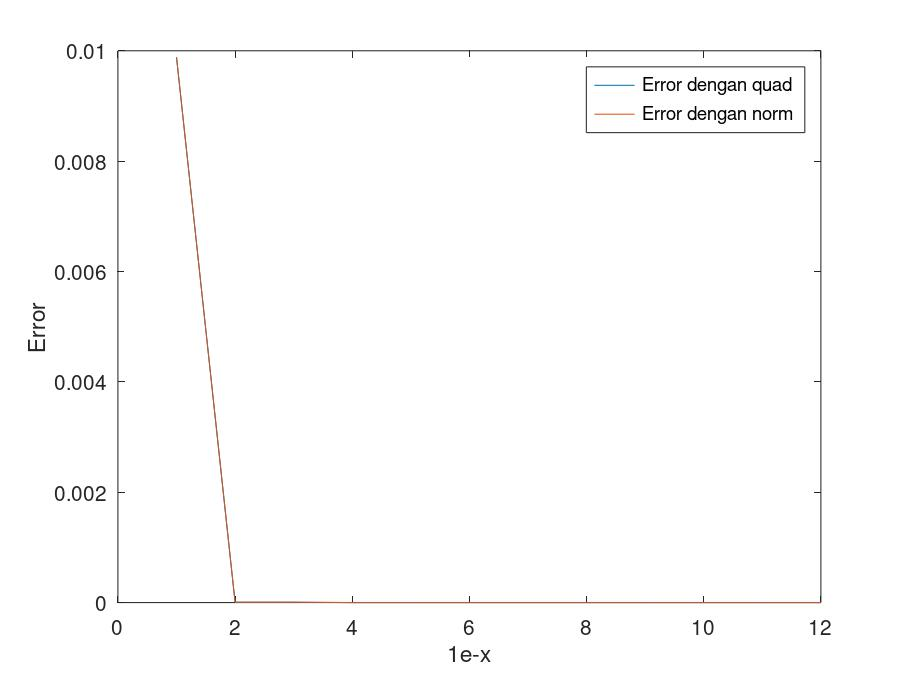
\includegraphics[width=0.5\textwidth]{quadnorm_romberg}
	\caption{Grafik Nilai Perbedaan antara Hasil Komputasi Romberg dan Fungsi Referensi}
	\label{fig:difGraph}
\end{figure}

Dari hasil analisis ini, bisa dijamin bahwa implementasi fungsi yang dilakukan menghasilkan hasil yang sesuai dan akurat, sesuai dengan batasan toleransi error dan memberikan hasil yang tidak jauh berbeda dengan fungsi referensi.

\subsection{Analisis Kompleksitas}
Kompleksitas dari fungsi dapat dilihat kembali melalui implementasi kode. Dalam TK ini, kompleksitas akan dihitung berdasarkan FLOP (\emph{floating-point operatons}) yang ada.
Pada implementasi yang dilakukan, akan dianalisis di luar \lstinline{for loop} yang ada.
\begin{center}
	\begin{lstlisting}[language=Octave]
if tol < 1e-14
	printf("Tolerance is too small and will produce errors, please use larger values\n")
	res = 0;
	return;
endif

n = 100;
R = zeros(n, n);
R(1,1) = (b-a)*(f(a)+f(b))/2;
	\end{lstlisting}
\end{center}

Di sini, terdapat 5 FLOPs yang terjadi, yaitu pada kondisi toleransi, dan inisiasi elemen pertama \\ \lstinline{R(1,1)}. Lanjut analisis ke dalam \emph{loop}
\begin{center}
	\begin{lstlisting}[language=Octave]
for j = 2:n
	h = (b-a)/2^(j-1);
	Rval = 0;

	for i = 1:2^(j-2)
		Rval = Rval + f(a+(2*i - 1)*h);
	endfor

		R(j,1) = (1/2)*R(j-1,1) + h*Rval;

	for k = 2:j
		topval = 4^(k-1)*R(j,k-1) - R(j-1,k-1);
		botval = 4^(k-1) - 1;
		R(j,k) = topval/botval;
	endfor

	if abs(R(j,j)-R(j-1,j-1)) < tol
		break;
	endif

endfor
	\end{lstlisting}
\end{center}

\par Pada bagian ini, di luar \lstinline{for loop} di dalam, terdapat 11 FLOPs, yaitu pada komputasi \lstinline{h}, menghitung \\ \lstinline{R(j,1)} dan mengecek batas toleransi, yang dijumlahkan menghasilkan kompleksitas FLOPs \(O(n)\)
Lalu, pada \lstinline{for loop} di dalam, terdapat 2 \lstinline{for loop} berbeda. Yang pertama, terdapat 5 FLOPs yang melakukan iterasi hingga \(2^{j-1}\) sehingga memiliki kompleksitas \(O(n*\log_2 j)\).
Untuk yang kedua, terdapat 11 FLOPs untuk iterasi sampai j dalam menghitung \lstinline{R(j,k)}, sehingga menghasilkan kompleksitas \(O(n*j)\). Dengan mengambil suku terbesar, maka kompleksitas dalam segi FLOPs untuk integrasi Romberg adalah \(O(n*j + n*\log_2 j)\).

Namun, kompleksitas juga bisa dihitung dalam segi \emph{function call}. Apabila kita ingin menghitung dalam segi ini, maka, melihat pada potongan kode di atas, di luar \lstinline{for loop} \emph{nested} terdapat 2 function call untuk menghitung \lstinline{R(1,1)}.
Lalu, pada \emph{nested loop} terdapat 1 \emph{function call} untuk iterasi \lstinline{Rval} dengan kompleksitas \(O(n*\log_2 j*(1))\). Jadi, untuk kompleksitas \emph{function call}, karena fungsi hanya dipanggil untuk menghitung dalam \emph{composite trapezoidal rule}, maka hanya dilakukan pada iterasi baris sebanyak \(log_2 (j-2)\) sehingga kompleksitas \emph{function call} hanya berupa \(O(n*\log_2 j)\).

Jika dilihat, kompleksitas implementasi Romberg bergantung pada \lstinline{j} dan \lstinline{n}, dengan \lstinline{j} bergantung pada \lstinline{n} karena tabel Romberg membentuk sebuah \emph{lower trianglular matrix}. Nilai \lstinline{n} ini merepresentasikan jumlah baris yang ada dan digunakan pada tabel/matriks Romberg, dengan implementasi di atas memiliki batas maksimum \lstinline{n = 100}.
Masalah yang dihadapi adalah menentukan jumlah \lstinline{n} yang eksak, karena algoritma Romberg berkembang secara dinamis tergantung pada fungsi dan toleransi, seperti yang dijelaskan pada bagian sebelumnya. Tetapi, aproksimasi dan tebakan kasar bisa dibentuk berdasarkan batas toleransi yang diberikan. Aproksimasi ini menggunakan teori yang disebutkan pada bagian sebelumnya, yaitu pertumbuhan akurasi \(O(h^{2k+2})\) dengan \(k\) adalah kolom ke-\(k\).
Jika kita memberikan suatu batas toleransi derajat-y atau \(10^{-y}\), maka kita bisa aproksimasi tabel yang dihasilkan akan berukuran \(O(h^{2k+2 = y})\) atau \(O(h^{k=\frac{y-2}{2}})\) dengan \(k\) adalah \(n\).
Sebuah percobaan dilakukan dengan premis ini. Menggunakan spesifikasi di awal, maka dibentuk grafik yang memetakan dari berbagai batas toleransi sehingga menghasilkan hasil berikut.

\begin{figure}[h]
	\centering
	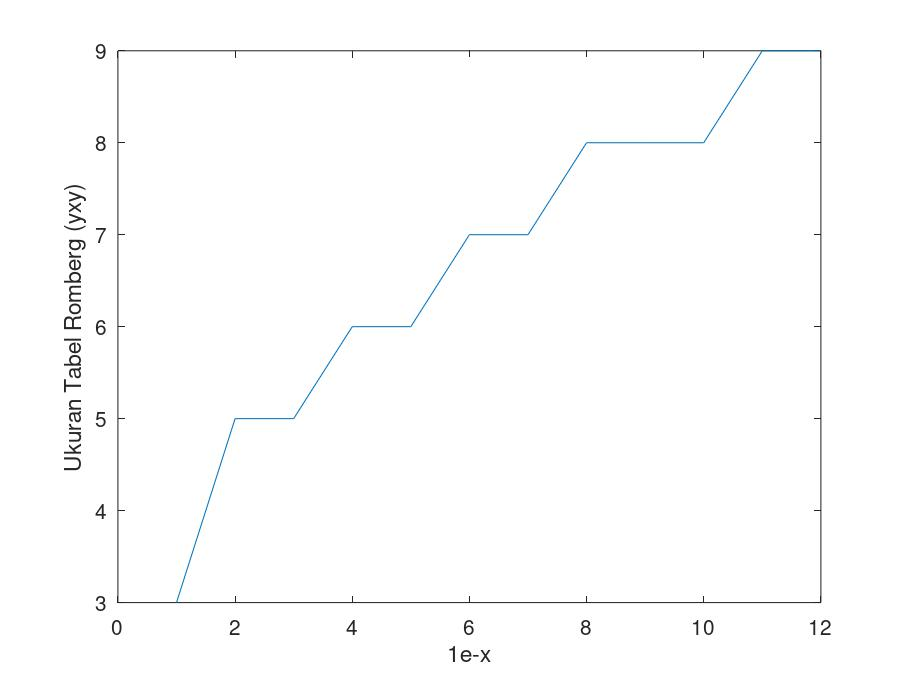
\includegraphics[width=0.5\textwidth]{rombergSize}
	\caption{Grafik Pertumbuhan Ukuran Tabel Romberg}
	\label{fig:rombergTableGraph}
\end{figure}
Dari hasil percobaan, ditemukan bahwa aproksimasi kasar tidak terlalu benar, namun hal yang jelas adalah tabel Romberg tumbuh secara fluktuatif tetapi sebanding mengikuti batas toleransi yang diberikan yang semakin kecil (artinya \emph{demand} akurasi meningkat dan perlu komputasi lebih intens yang mengakibatkan tabel Romberg semakin besar).
Salah satu perkiraan alasan mengapa terjadi seperti ini adalah tipe fungsi yang diberikan, seperti yang disebutkan pada bagian sebelumnya di mana tipe fungsi yang digunakan akan memengaruhi akurasi dan seberapa banyak komputasi yang perlu dilakukan.
Maka dari itu, bisa disimpulkan bahwa kompleksitas secara kasar untuk komputasi FLOPs adalah \(O(n*j + n*\log_2 j)\) dan untuk \emph{function call} adalah \(O(n*\log_2 j)\) dengan \(n\) adalah ukuran tabel Romberg yang bergantung pada fungsi dan batas toleransi serta nilai masukan, dan \(j\) bergantung pada \(n\).


\subsection{Analisis Kompleksitas}
Kompleksitas dari fungsi dapat dilihat kembali melalui implementasi kode. Dalam TK ini, kompleksitas akan dihitung berdasarkan FLOP (\emph{floating-point operatons}) yang ada.
Pada implementasi yang dilakukan, akan dianalisis di luar \lstinline{for loop} yang ada.
\begin{center}
	\begin{lstlisting}[language=Octave]
if tol < 1e-14
	printf("Tolerance is too small and will produce errors, please use larger values\n")
	res = 0;
	return;
endif

n = 100;
R = zeros(n, n);
R(1,1) = (b-a)*(f(a)+f(b))/2;
	\end{lstlisting}
\end{center}

Di sini, terdapat 5 FLOPs yang terjadi, yaitu pada kondisi toleransi, dan inisiasi elemen pertama \\ \lstinline{R(1,1)}. Lanjut analisis ke dalam \emph{loop}
\begin{center}
	\begin{lstlisting}[language=Octave]
for j = 2:n
	h = (b-a)/2^(j-1);
	Rval = 0;

	for i = 1:2^(j-2)
		Rval = Rval + f(a+(2*i - 1)*h);
	endfor

		R(j,1) = (1/2)*R(j-1,1) + h*Rval;

	for k = 2:j
		topval = 4^(k-1)*R(j,k-1) - R(j-1,k-1);
		botval = 4^(k-1) - 1;
		R(j,k) = topval/botval;
	endfor

	if abs(R(j,j)-R(j-1,j-1)) < tol
		break;
	endif

endfor
	\end{lstlisting}
\end{center}
Pada bagian ini, di luar \lstinline{for loop} di dalam, terdapat 11 FLOPs, yaitu pada komputasi \lstinline{h}, menghitung \lstinline{R(j,1)} dan mengecek batas toleransi, yang dijumlahkan menghasilkan kompleksitas FLOPs \(O(n)\)
Lalu, pada \lstinline{for loop} di dalam, terdapat 2 \lstinline{for loop} berbeda. Yang pertama, terdapat 5 FLOPs yang melakukan iterasi hingga \(2^{j-1}\) sehingga memiliki kompleksitas \(O(n*\log_2 j)\).
Untuk yang kedua, terdapat 11 FLOPs untuk iterasi sampai j dalam menghitung \lstinline{R(j,k)}, sehingga menghasilkan kompleksitas \(O(n*j)\). Dengan mengambil suku terbesar, maka kompleksitas dalam segi FLOPs untuk integrasi Romberg adalah \(O(n*j + n*\log_2 j)\).

Namun, kompleksitas juga bisa dihitung dalam segi \emph{function call}. Apabila kita ingin menghitung dalam segi ini, maka, melihat pada potongan kode di atas, di luar \lstinline{for loop} \emph{nested} terdapat 2 function call untuk menghitung \lstinline{R(1,1)}.
Lalu, pada \emph{nested loop} terdapat 1 \emph{function call} untuk iterasi \lstinline{Rval} dengan kompleksitas \(O(n*\log_2 j*(1))\). Jadi, untuk kompleksitas \emph{function call}, karena fungsi hanya dipanggil untuk menghitung dalam \emph{composite trapezoidal rule}, maka hanya dilakukan pada iterasi baris sebanyak \(log_2 (j-2)\) sehingga kompleksitas \emph{function call} hanya berupa \(O(n*\log_2 j)\).

Jika dilihat, kompleksitas implementasi Romberg bergantung pada \lstinline{j} dan \lstinline{n}, dengan \lstinline{j} bergantung pada \lstinline{n} karena tabel Romberg membentuk sebuah \emph{lower trianglular matrix}. Nilai \lstinline{n} ini merepresentasikan jumlah baris yang ada dan digunakan pada tabel/matriks Romberg, dengan implementasi di atas memiliki batas maksimum \lstinline{n = 100}.
Masalah yang dihadapi adalah menentukan jumlah \lstinline{n} yang eksak, karena algoritma Romberg berkembang secara dinamis tergantung pada fungsi dan toleransi, seperti yang dijelaskan pada bagian sebelumnya. Tetapi, aproksimasi dan tebakan kasar bisa dibentuk berdasarkan batas toleransi yang diberikan. Aproksimasi ini menggunakan teori yang disebutkan pada bagian sebelumnya, yaitu pertumbuhan akurasi \(O(h^{2k+2})\) dengan \(k\) adalah kolom ke-\(k\).
Jika kita memberikan suatu batas toleransi derajat-y atau \(10^y\), maka kita bisa aproksimasi tabel yang dihasilkan akan berukuran \(O(h^{2k+2 = y})\) atau \(O(h^{k=\frac{y-2}{2}})\) dengan \(k\) adalah \(n\).
Sebuah percobaan dilakukan dengan premis ini. Menggunakan spesifikasi di awal, maka dibentuk grafik yang memetakan dari berbagai batas toleransi sehingga menghasilkan hasil berikut.

\begin{figure}[h]
	\centering
	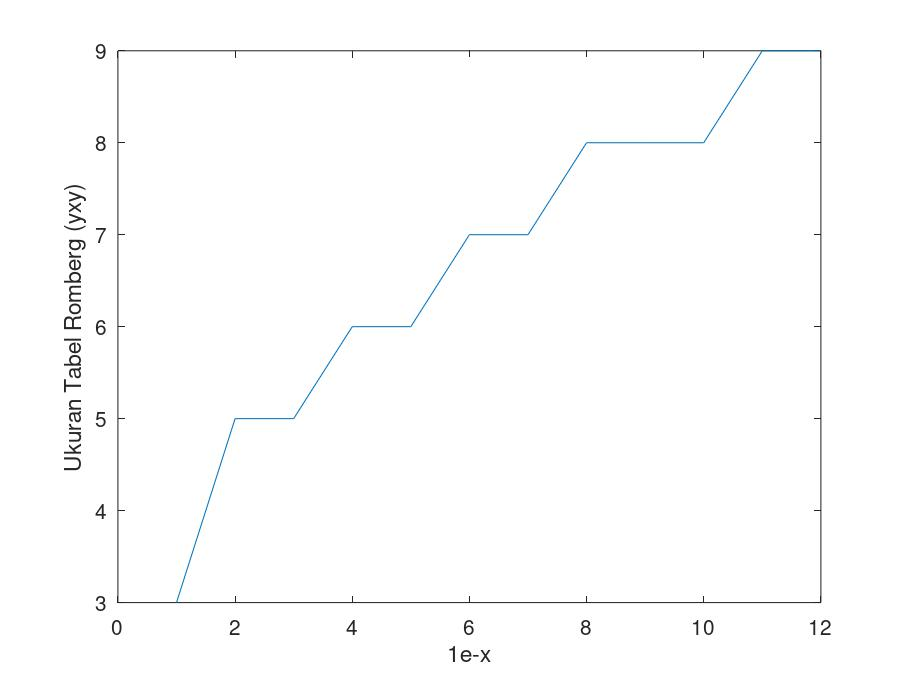
\includegraphics[width=0.5\textwidth]{rombergSize}
	\caption{Grafik Pertumbuhan Ukuran Tabel Romberg}
	\label{fig:rombergTableGraph}
\end{figure}
Dari hasil percobaan, ditemukan bahwa aproksimasi kasar tidak terlalu benar, tetapi hal yang jelas adalah tabel Romberg tumbuh secara fluktuatif tetapi sebanding mengikuti batas toleransi yang diberikan yang semakin kecil (artinya \emph{demand} akurasi meningkat dan perlu komputasi lebih intens yang mengakibatkan tabel Romberg semakin besar).
Salah satu perkiraan alasan mengapa terjadi seperti ini adalah tipe fungsi yang diberikan, seperti yang disebutkan pada bagian sebelumnya di mana tipe fungsi yang digunakan akan memengaruhi akurasi dan seberapa banyak komputasi yang perlu dilakukan.
Maka dari itu, bisa disimpulkan bahwa kompleksitas secara kasar untuk komputasi FLOPs adalah \(O(n*j + n*\log_2 j)\) dan untuk \emph{function call} adalah \(O(n*\log_2 j)\) dengan \(n\) adalah ukuran tabel Romberg yang bergantung pada fungsi dan batas toleransi serta nilai masukan, dan \(j\) bergantung pada \(n\).

\section{Kesimpulan}
Kesimpulan disini.

% % Example of a table from http://www.latextemplates.com/template/professional-table

\begin{thebibliography}{1}
	% Here are a few examples of different citations 
	% Book
	\bibitem{kopka_1999} % Note the label in the curly brackets. Use the cite the source; e.g., \cite{kopka_latex}
	H.~Kopka and P.~W. Daly, \emph{A Guide to \LaTeX}, 3rd~ed.\hskip 1em plus
	0.5em minus 0.4em\relax Harlow, England: Addison-Wesley, 1999.
	\bibitem{horowitz_2005}D.~Horowitz, \emph{End of Time}. New York, NY, USA: Encounter Books, 2005. [E-book] Available: Ebrary, \url{http://site.ebrary.com/lib/sait/Doc?id=10080005}. Accessed on: Oct. 8, 2008.

	% Article from database
	\bibitem{castlevecchi_2008}D.~Castelvecchi, ``Nanoparticles Conspire with Free Radicals'' \emph{Science News}, vol.174, no. 6, p. 9, September 13, 2008. [Full Text]. Available: Proquest, \url{http://proquest.umi.com/pqdweb?index=52&did=1557231641&SrchMode=1&sid=3&Fmt=3&VInst=PROD&VType=PQD&RQT=309&VName=PQD&TS=1229451226&clientId=533}. Accessed on: Aug.~3, 2014.
	% Conference Paper from the Internet
	\bibitem{lach_2010}J.~Lach, ``SBFS: Steganography based file system,'' in \emph{Proceedings of the 2008 1st International Conference on Information Technology, IT 2008, 19-21 May 2008, Gdansk, Poland.} Available: IEEE Xplore, \url{http://www.ieee.org}. [Accessed: 10 Sept. 2010].
	% Web page, no author
	\bibitem{a_laymans_explanation}``A `layman's' explanation of Ultra Narrow Band technology,'' Oct.~3, 2003. [Online]. Available: \url{http://www.vmsk.org/Layman.pdf}. [Accessed: Dec.~3, 2003].
	=======
	\bibitem{jim_lamber}Jim Lambers, \emph{Lecture 29 Notes}.
	Mississippi, USA: University of Southern Mississippi, 2009. [MAT 460/560 Fall Semester 2009-10 Lecture Notes] Available: math.usm.edu, \url{https://www.math.usm.edu/lambers/mat460/fall09/lecture29.pdf}. Accessed on: Dec. 17, 2022.
\end{thebibliography}

% This is a hand-made bibliography. If you want to use a BibTeX file, you're on your own ;-)














\end{document}